%-*- coding: utf-8 -*-
\label{chap:erm}

\paragraph{Notions :} classification, régression, espace des hypothèses,
minimisation du risque empirique, modèles paramétriques
linéaires, moindres carrés
\paragraph{Objectifs pédagogiques :} 
\begin{itemize}      
  \setlength{\itemsep}{3pt}
\item Formaliser un problème d'apprentissage supervisé.
\item Décrire l'espace des hypothèses dans le cas d'un modèle paramétrique.
\item Prouver l'équivalence entre maximisation de la vraisemblance et
  minimisation du risque empirique dans le cas gaussien. $\bullet$ 
\item Mettre en \oe{}uvre une régression linéaire.
\end{itemize}

Nous nous intéressons maintenant aux problèmes d'apprentissage \textbf{supervisé}
: il s'agit de développer des algorithmes qui soient capables d'apprendre des
modèles \textbf{prédictifs}. À partir d'exemples étiquetés, ces modèles seront
capables de prédire l'étiquette de nouveaux objets. Le but de ce chapitre est
de développer les concepts généraux qui nous permettent de formaliser ce type
de problèmes.

\section{Formalisation d'un problème d'apprentissage supervisé}
\label{sec:sup_learn}
Nous supposons maintenant disposer non seulement d'une matrice
$X \in \RRnp$ décrivant $n$ individus en $p$ dimensions, mais aussi
de $n$ \textbf{étiquettes} $\{y^1, y^2, \dots, y^n\}$. Chaque étiquette $y^i$
appartient à un espace $\YY.$ Dans ce cours, nous allons considérer deux cas
particuliers pour $\YY:$
\begin{itemize}
\item $\YY = \RR :$ on parle d'un problème de \textbf{régression} ;
\item $\YY = \zo :$ on parle d'un problème de \textbf{classification
    binaire}, et les observations dont l'étiquette vaut $0$ sont appelées
  \textbf{négatives} tandis que celles dont l'étiquette vaut $1$ sont appelées
  \textbf{positives}. Dans certains cas, il sera mathématiquement plus simple
  d'utiliser $\YY = \mopo$.
\end{itemize}

La matrice $X \in \RRnp$ telle que $X_{ij} = x^i_j$ est la $j$-ème
variable du $i$-ème individu est appelée \textbf{matrice de données} ou
\textbf{matrice de design}. 

On peut aussi choisir de représenter chaque individu et son étiquette par le
couple $(\xx^i, y^i) \in \RR^{p} \times \YY.$ L'ensemble
$\DD = \{(\xx^i, y^i)\}_{i=1, \dots, n}$ forme alors le \textbf{jeu d'apprentissage}.

Le machine learning étant issu de plusieurs disciplines et champs
d'applications, on trouvera plusieurs noms pour les mêmes objets.  Ainsi les
variables sont aussi appelées \textbf{descripteurs}, \textbf{attributs},
\textbf{prédicteurs}, ou \textbf{caractéristiques} (en anglais,
\textit{variables, descriptors, attributes, predictors} ou encore
\textit{features}).  Les \textbf{individus}, ou \textbf{observations} sont
aussi appelées \textbf{exemples}, \textbf{échantillons} ou \textbf{points du
  jeu de données} (en anglais, \textit{samples} ou \textit{data
  points}). Enfin, les étiquettes sont aussi appelées \textbf{variables cibles}
(en anglais, \textit{labels, targets} ou \textit{outcomes}).

% Ces concepts sont illustrés sur la figure~\ref{fig:suplearning}.

% \begin{figure}[h]
%   \centering
%   \includegraphics[width=0.7\textwidth]{figures/erm/suplearning}
%   \caption{Les données d'un problème d'apprentissage supervisé sont organisées
%     en une matrice de design et un vecteur d'étiquettes. Les observations sont
%     représentées par leurs variables explicatives.}
%   \label{fig:suplearning}
% \end{figure}

Le but de l'apprentissage supervisé est alors de trouver une fonction
$f: \RR^p \to \YY$ telle que $f(\xx) \approx y,$ qui s'applique non
seulement aux $n$ individus observés, mais plus généralement à tous les
individus d'une population à laquelle on suppose que ces $n$ individus
appartiennent. C'est cette fonction $f$ qui est le \textbf{modèle prédictif}
appris. Un \textbf{algorithme d'apprentissage supervisé} utilise le jeu de
données $\DD$ pour déterminer $f$.

Plus formellement, supposons que les couples $(\xx^i, y^i)$ soient les
réalisations de $n$ vecteurs aléatoires de même loi qu'un couple de variables
aléatoire $(X, Y)$, $X$ étant un vecteur aléatoire à $p$ dimensions et $Y$ une
variable aléatoire réelle à valeurs dans $\YY$. Supposons de plus qu'il existe
une fonction $\Phi \colon \RR^p \to \YY$ et une variable aléatoire réelle
$\epsilon$ telle que
  \begin{equation}
  Y = \Phi(X) + \epsilon,
  \label{eq:probabilistic_ml}
\end{equation}
$\epsilon$ représentant un \textbf{bruit}.
Ce bruit peut être causé
\begin{itemize}
\item par des {\it erreurs de mesure} dues à la faillibilité des capteurs
  utilisés pour mesurer les variables par lesquelles on représente nos
  données, ou à la faillibilité des personnes qui ont entré ces
  mesures dans une base de données ;
\item par des {\it erreurs d'étiquetage} (souvent appelés {\it teacher's noise}
  en anglais) dues à la faillibilité des personnes qui ont étiqueté
  les données ;
\item enfin, parce que les variables mesurées ne suffisent pas à modéliser le
  phénomène qui nous intéresse, soit qu'on ne les connaisse pas, soit
  qu'elles soient coûteuses à mesurer.
\end{itemize}
Notre but est d'approcher $\Phi$ par $f$.

Dans le cas d'un problème de classification, le modèle prédictif peut prendre
directement la forme d'une fonction $f$ à valeurs dans $\zo$, ou utiliser
une fonction intermédiaire $g$ à valeurs réelles, qui associe à une observation
un score d'autant plus élevé qu'elle est susceptible d'être positive. Ce score
peut par exemple être la probabilité que cette observation appartienne à la
classe positive. On obtient alors $f$ en \textbf{seuillant} $g$ ; $g$ est
appelée \textbf{fonction de décision} \footnote{Dans la librairie
  \texttt{scikit-learn}, on fera ainsi attention à la distinction entre les
  méthodes \texttt{predict} et \texttt{predict\_proba}.}.

\begin{exemple}
  \paragraph{Filtrage de spam.} On peut poser le filtrage de spam comme un
  problème de classification binaire. Les individus sont des emails. Leur
  étiquette est binaire (positive pour « spam » et négative pour « non-spam
  »). Les $p$ variables représentant un email peuvent être définies comme le
  nombre d'occurrences, pour $p$ mots, de chacun de ces mots dans l'email ($p$
  est ainsi la taille d'un dictionnaire pré-défini)\footnote{C'est ce qu'on
    appelle une représentation \textit{bag-of-words}}. Étant donné un jeu de
  données de $n$ emails étiquetés, un algorithme d'apprentissage retourne une
  fonction $f$ qui, à tout email représenté par un vecteur de $\RR^p$ (en fait,
  $\NN^p$), associe une étiquette $0$ ou $1$. Ce modèle
  $f: \RR^p \to \zo$ peut être obtenu en seuillant une fonction de
  décision $g: \RR^p \to \RR$.

  Le bruit peut être dû aux causes suivantes :
  \begin{itemize}
  \item Des erreurs de mesures peuvent être causées par des fautes
    d'orthographe (volontaires ou non) qui empêchent de comptabiliser certains
    mots.
  \item Des erreurs d'étiquetage peuvent arriver quand une personne marque par
    erreur comme courrier indésirable un email qui ne l'était pas, ou,
    inversement, laisse dans sa boîte mail ou supprime sans étiqueter comme tel
    un email indésirable.
  \item Enfin, notre représentation est limitée, en particulier parce qu'elle
    ne considère pas l'ordre des mots. Nous ne disposons pas de suffisamment
    d'information pour classifier les emails aussi efficacement qu'un humain.
  \end{itemize}
\end{exemple}


\paragraph{Remarque.} Les notions développées jusqu'à la fin de la
section~\ref{sec:losses} peuvent l'être en remplaçant $\RR^p$ par un espace
quelconque $\XX$.


\section{Espace des hypothèses}
Pour poser un problème d'apprentissage supervisé, il nous faut décider du
type de modèles que nous allons considérer. 

On appelle \textbf{espace des hypothèses} l'espace de fonctions $\FF$, qui est
un sous-espace de toutes les fonctions de $\RR^p \to \YY$ décrivant les
modèles que nous allons considérer. Cet espace est choisi en
fonction de nos {\it convictions} par rapport au problème, ainsi que de
considérations pratiques sur notre capacité à trouver facilement un « bon »
modèle dans $\FF$.

Le choix de l'espace des hypothèses est fondamental.  En effet, si cet espace
ne contient pas le \og bon \fg~modèle, il sera impossible de trouver une bonne
fonction de décision.  Cependant, si l'espace est trop générique, il sera plus
difficile et intensif en temps de calcul d'y trouver un bon modèle.
  

\begin{exemple}
  Dans l'exemple de la figure~\ref{fig:simple_classif_pb}, on pourra décider de
  se restreindre à des discriminants qui soient des ellipses à axes parallèles
  aux axes de coordonnées.  Ainsi, l'espace des hypothèses sera
  \begin{equation}
    \FF = \{ \xx \mapsto \alpha (x_1-a)^2 + \beta (x_2-b)^2 - 1 \; ; (\alpha, \beta, a, b) \in \RR^4\}.
    \label{eq:hypothesis_space_ellipsis}
  \end{equation}

  Dans cet espace, il semble possible de trouver un modèle $f$ qui sépare les
  positifs des négatifs. Si nous avions choisi comme espace des hypothèses
  l'ensemble des fonctions linéaires de $\RR^2$ dans $\RR$, ce ne serait pas
  possible.
\end{exemple}
\begin{figure}[h]
  \centering
  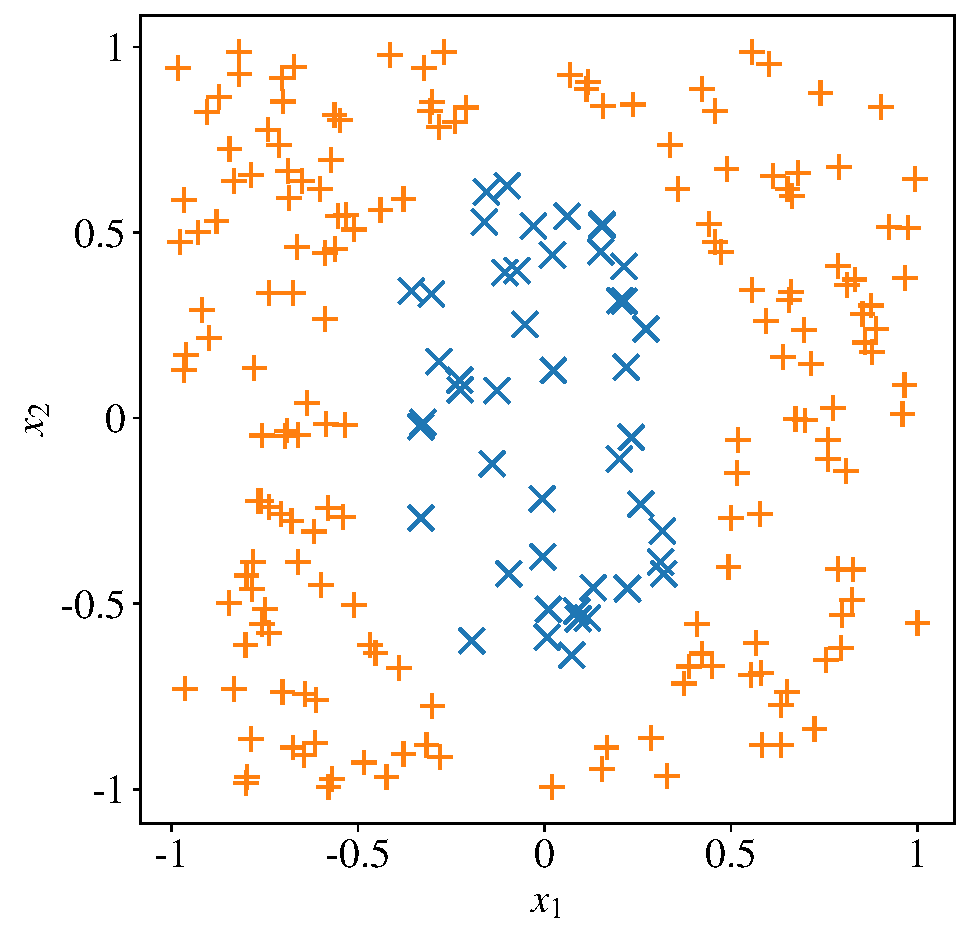
\includegraphics[width=0.45\textwidth]{figures/erm/simple_classif}
  \caption{Les exemples positifs (+) et négatifs (x) semblent être séparables
    par une ellipse.}
  \label{fig:simple_classif_pb}
\end{figure}

La tâche d'apprentissage supervisé consiste à déterminer une hypothèse
$f \in \FF$ qui approche au mieux la fonction cible $\Phi$ (voir
équation~\eqref{eq:probabilistic_ml}). Pour réaliser une telle tâche, nous
allons développer dans les sections suivantes deux outils supplémentaires :
\begin{enumerate}
\item Une façon de \textbf{quantifier la qualité d'une hypothèse}, afin de
  pouvoir déterminer si une hypothèse satisfaisante (voire optimale) a été
  trouvée.  Pour cela, nous allons définir la notion de \textbf{fonction de
    coût}.
\item Une façon de \textbf{chercher une hypothèse optimale} dans $\FF$.  Les
  algorithmes d'apprentissage supervisé que nous allons étudier ont pour but de
  trouver dans $\FF$ l'hypothèse optimale au sens de la fonction de coût. Selon
  les cas, et en particulier selon le choix de $\FF,$ cette recherche sera
  exacte ou approchée.
\end{enumerate}

\section{Minimisation du risque empirique}
\label{sec:mre}
Résoudre un problème d'apprentissage supervisé revient à trouver une fonction
$f \in \FF$ dont les prédictions soient les plus proches possibles des
véritables étiquettes, sur tout l'espace $\RR^p$. On utilise pour formaliser cela
la notion de \textbf{fonction de coût} :

Une \textbf{fonction de coût} $L: \YY \times \YY \to \RR$, 
aussi appelée \textbf{fonction de perte} ou \textbf{fonction d'erreur}
(en anglais : {\it cost function} ou {\it loss function})
est une fonction utilisée pour quantifier la qualité d'une prédiction : 
$L(y, f(\xx))$ est d'autant plus grande que l'étiquette $f(\xx)$ est éloignée de
la vraie valeur $y$.

Étant donnée une fonction de coût $L$, nous cherchons donc $f$ qui minimise ce
coût sur l'ensemble des valeurs possibles de $\xx \in \RR^p$, ce qui est
formalisé par la notion de \textbf{risque.} Nous supposons que les couples
$(\xx^i, y^i)$ sont les réalisations de $n$ vecteurs aléatoires de même loi
qu'un couple de variables aléatoire $(X, Y).$

Dans le cadre d'un problème d'apprentissage supervisé, on appelle
\textbf{risque} d'un modèle $h$ l'espérance de son coût :
\begin{equation}
  \label{eq:risque}
  \Rcal(h) = \EE(L(Y, f(X))).
\end{equation}

Nous cherchons donc un modèle $f$ tel que 
\begin{equation}
  \label{eq:risk_minimization}
  f \in \argmin_{h \in \FF} \EE(L(Y, h(X))).
\end{equation}
Ce problème est généralement insoluble sans plus d'hypothèses : nous ne
connaissons que $n$ réalisations du couple $(X, Y)$.  On approchera donc le
risque par son estimation sur ces réalisations.

On appelle \textbf{risque empirique} de $h$ l'estimée du risque de $h$ défini par
\begin{equation}
  \label{eq:empirical_risk}
  R_n(h) = \frac{1}{n} \sum_{i=1}^n L(y^i, h(\xx^i)).
\end{equation}

On appelle donc modèle obtenu par \textbf{minimisation du risque empirique} une
fonction
\begin{equation}
  \label{eq:erm}
  f \in \argmin_{h \in \FF} \frac{1}{n} \sum_{i=1}^n L(y^i, h(\xx^i)).
\end{equation}

Selon le choix de $\FF$ et $L$, l'équation~\ref{eq:erm} peut avoir une solution
analytique explicite. Cela ne sera pas souvent le cas ; cependant on choisira
souvent une fonction de coût convexe afin de résoudre plus facilement ce
problème d'optimisation.

La minimisation du risque empirique est généralement un problème {\it mal
  posé}, c'est-à-dire qu'il n'admet pas une solution unique dépendant de façon
continue de conditions initiales. Il se peut par exemple qu'un nombre infini
de solutions minimise le risque empirique à zéro (voir
figure~\ref{fig:multiple_solutions}).

\begin{figure}[h]
  \centering
  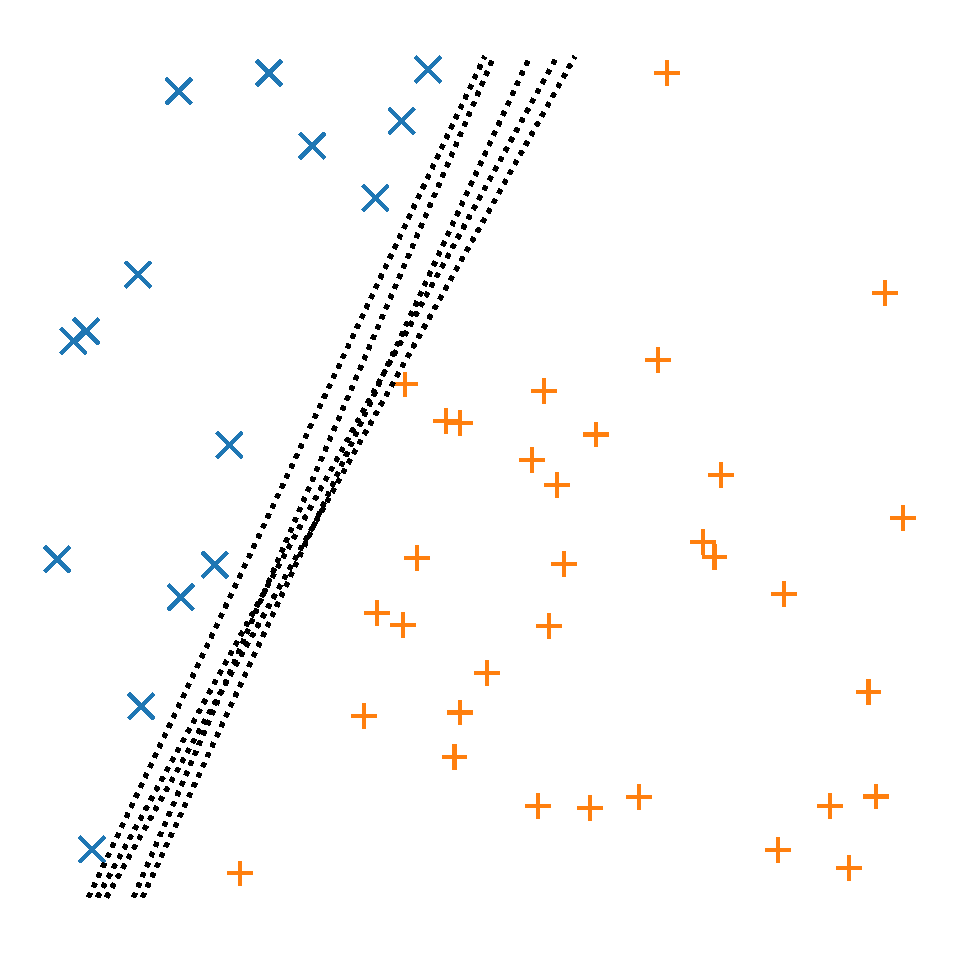
\includegraphics[width=0.4\textwidth]{figures/erm/multiple_solutions}
  \caption{Une infinité de droites séparent parfaitement les points positifs
    (+) des points négatifs (x). Chacune d'entre elles a un risque empirique
    nul.}
  \label{fig:multiple_solutions}
\end{figure}


\paragraph{Convergence} La loi des grands nombres nous garantit que le risque
empirique d'un modèle $h \in \FF$ converge vers le risque quand la taille de
l'échantillon tend vers l'infini :
\begin{equation}
  \label{eq:risk_cvg}
  R_n(h) \xrightarrow[n \to \infty]{} \Rcal(h).
\end{equation}
Cela ne suffit cependant pas à garantir que le minimum du risque empirique
$\min_{h \in \FF} R_n(h)$ converge vers le minimum du risque
$\min_{h \in \FF} \Rcal(h)$. En effet, si $\FF$ est l'espace des fonctions
mesurables, le minimiseur de $R_n(h)$ vaut généralement $0$, ce qui n'est pas
le cas de $\Rcal(h).$ \textbf{Il n'y a donc aucune garantie qu'un modèle qui
  minimise le risque empirique minimise le risque.} C'est une remarque très
importante car elle signifie que le fait qu'un modèle minimise l'erreur sur nos
$n$ observations ne donne aucune garantie quant à sa performance sur d'autres
observations. Nous reviendrons sur ce sujet lors du prochain chapitre, en abordant
les notions de généralisation et de surapprentissage.

La convergence de la minimisation du risque empirique dépend de $\FF$. L'étude
de cette convergence est l'un des principaux éléments de la théorie de
l'apprentissage de Vapnik-Chervonenkis, qui dépasse largement le cadre de ce
cours.


\section{Fonctions de coût}
\label{sec:losses}
Il existe de nombreuses fonctions de coût. Le choix d'une fonction de coût
dépend d'une part du problème en lui-même, autrement dit de ce que l'on trouve
pertinent pour le cas pratique considéré, et d'autre part de considérations
pratiques : peut-on ensuite résoudre le problème d'optimisation qui résulte de
ce choix de façon suffisamment exacte et rapide~?
Cette section présente quelques-unes des fonctions de coût les plus utilisées.

\subsection{Coût 0/1 (classification)}
Dans le cas d'une fonction $f$ à valeurs discrètes, on appelle \textbf{fonction
  de coût 0/1}, ou {\it 0/1 loss}, la fonction suivante :
\begin{align*}
  L_{0/1}\colon\YY \times \YY & \to \RR \\
  y, f(\xx) & \mapsto
              \begin{cases}
                1 & \mbox{ si } f(\xx) \neq y \\
                0 & \mbox{ sinon.}
              \end{cases}
\end{align*}
Le risque empirique d'un modèle $h$ sur un jeu de données est alors le nombre
d'erreurs de prédiction sur ce jeu de données.

\subsection{Coût logistique et entropie croisée (classification binaire)}
Considérons maintenant que $f$ est une fonction de décision à valeurs réelles.
\label{sec:logistic_loss}
On appelle \textbf{fonction de coût logistique}, ou {\it logistic loss}, la
fonction suivante :
\begin{equation}
  \begin{split}
  L_{\log}\colon\mopo \times \RR & \to \RR \\ 
  y, f(\xx) & \mapsto \ln \left( 1 + \exp(-y f(\xx))\right). 
\end{split}
  \label{eq:logistic_loss}
\end{equation}

Si $f$ est à valeurs dans $]0, 1[$, en particulier si $f(\xx)$ est la
probabilité que $\xx$ appartienne à la classe positive, % cette fonction de coût
% est équivalente à
on utilise plutôt
l'\textbf{entropie croisée}, définie pour $\YY = \zo$.

\label{sec:cross_entropy}
On appelle \textbf{entropie croisée}, ou {\it cross-entropy},
la fonction suivante :
\begin{equation}
  \begin{split}
    L_H \colon \zo \times ]0, 1[ & \to \RR \\
    y, f(\xx) & \mapsto - y \ln f(\xx) - (1-y) \ln(1-f(\xx)).
  \end{split}
  \label{eq:cross_entropy}
\end{equation}

\paragraph{Remarque} On peut transformer une fonction $f$ à valeurs dans $\RR$
en une fonction $h$ à valeurs dans $]0, 1[$ en la composant par la
\textbf{fonction sigmoïde,} aussi appelée \textbf{fonction logistique,} définie
par
\begin{equation}
  \label{eq:sigmoide}
  \begin{split}
    \sigma \colon \RR & \to ]0, 1[ \\
    u & \mapsto \frac1{1 + e^{-u}}.
  \end{split}
\end{equation}
Dans ce cas, la fonction de coût logistique appliquée à $f$ est équivalente à
l'entropie croisée appliquée à $h = \sigma \circ f$ :
\[
  L_H(y, h(\xx)) = L_{\log} (2y-1, f(\xx))
\]

La figure~\ref{fig:logistic_loss} illustre la valeur de la fonction de coût
logistique en fonction de l'étiquette $y$ de l'individu $\xx$ et de la valeur
de la fonction de décision $f(\xx) \in ]0, 1[.$ 

\begin{figure}[h]
  \centering
  \begin{subfigure}[t]{0.43\textwidth}
    \centering
    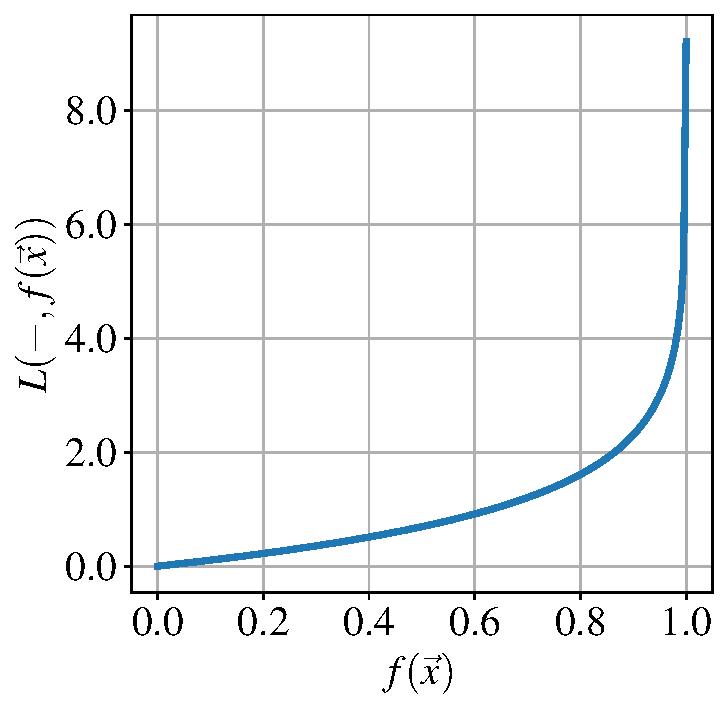
\includegraphics[width=\textwidth]{figures/erm/logistic_loss_neg}
    \caption{Entropie croisée pour un individu d'étiquette négative, en
      fonction de la valeur de la fonction de décision. Cette perte est
      d'autant plus grande que la fonction de décision est proche de $1$.}
    \label{fig:logistic_loss_neg}
  \end{subfigure} \hfill
  \begin{subfigure}[t]{0.43\textwidth}
    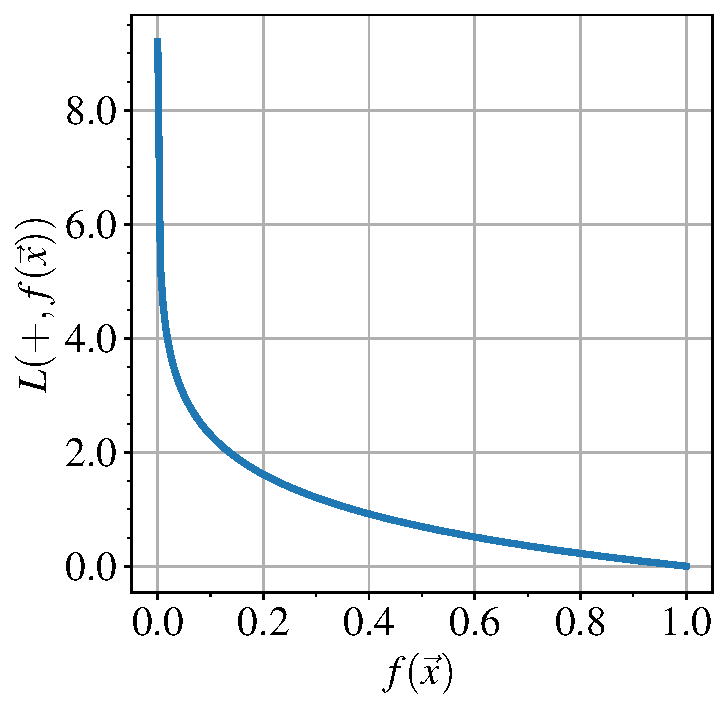
\includegraphics[width=\textwidth]{figures/erm/logistic_loss_pos}  
    \caption{Entropie croisée pour un individu d'étiquette positive, en
      fonction de la valeur de la fonction de décision. Cette perte est
      d'autant plus grande que la fonction de décision est proche de $0$.}
    \label{fig:logistic_loss_pos}
  \end{subfigure}
  \caption{Valeur de l'entropie croisée en fonction de la valeur de la fonction de décision.}
  \label{fig:logistic_loss}
\end{figure}


\paragraph{Pourquoi « entropie croisée » ? $\bullet\bullet$ } 
L'entropie croisée est issue de la théorie de l'information, d'où son nom. En
considérant que la véritable classe d'une observation est modélisée par une
distribution $Q$, et sa classe prédite est modélisée par une distribution $P$,
nous allons chercher à modéliser $P$ de sorte qu'elle soit la plus proche
possible de $Q$. On utilise pour cela la divergence de Kullback-Leibler,
définie par :
\begin{align*}
  \text{KL}(Q||P) & = \sum_{c=0, 1} Q(Y=c|X) \ln \frac{Q(Y=c|X)}{P(Y=c|X)} \\
           & = - \sum_{c=0, 1} Q(Y=c|X) \ln P(Y=c|X) + 
             \sum_{c=0, 1} Q(Y=c|X) \ln Q(Y=c|X).
\end{align*}
Comme $Q(Y=c|X)$ vaut soit $0$ ($c$ n'est pas la classe de $X$) soit
$1$ (dans le cas contraire), le deuxième terme de cette expression est nul
et on retrouve ainsi la définition ci-dessus de l'entropie croisée.

\subsection{Coût quadratique (régression)}
\label{sec:quadratic_loss}
On appelle \textbf{fonction de coût quadratique}, ou {\it quadratic loss}, ou
{\it squared error}, la fonction suivante :
\begin{equation}
  \begin{split}
    L_{\text{SE}}\colon\RR \times \RR & \to \RR \\ 
    y, f(\xx) & \mapsto \frac12 \left(y - f(\xx)\right)^2.
\end{split}
  \label{eq:quadratic_loss}  
\end{equation}
Le coefficient $\frac{1}{2}$ permet d'éviter d'avoir des coefficients
multiplicateurs quand on dérive le risque empirique pour le minimiser.

\section{Apprentissage supervisé d'un modèle de régression paramétrique}
\label{sec:parametric}
\subsection{Modèles paramétriques}
On parle de \textbf{modèle paramétrique} quand l'espace des hypothèses $\FF$
est un ensemble de fonctions définies par une expression analytique
paramétrisée par un nombre fini de paramètres. 

C'est le cas de l'espace des hypothèses défini plus haut par
l'équation~\eqref{eq:hypothesis_space_ellipsis} : les paramètres sont au nombre
de $4$ et il s'agit de $\alpha$, $\beta$, $a$, et $b$. Le but de
l'apprentissage sera de déterminer les valeurs de ces paramètres.  À l'inverse,
la méthode du plus proche voisin, qui associe à $\xx$ l'étiquette du point du
jeu d'entraînement dont il est le plus proche en distance euclidienne, apprend
un modèle non paramétrique : il ne s'agit pas d'écrire la fonction de décision
comme une expression explicite des variables prédictives et d'apprendre les
paramètres de cette expression. Nous verrons au chapitre~\ref{chap:nonlin}
d'autres exemples de modèles non paramétriques.
% , et nous concentrons maintenant sur les modèles de régression
% paramétriques. 
Nous considérons pour la suite de ce chapitre disposer d'un jeu
$\DD = \{\xx^i, y^i\}_{i=1, \dots, n}$ de $n$ observations en $p$ dimensions et
leurs étiquettes réelles. Nous considérons comme espace des hypothèses un
ensemble de modèles paramétrisés par un vecteur $\bbeta \in \mathbb{R}^{m}$.


\subsection{Minimisation du risque empirique d'une régression paramétrique}
Si nous utilisons comme fonction de coût le coût quadratique défini par
l'équation~\eqref{eq:quadratic_loss}, la minimisation du risque empirique comme
définie par l'équation~\eqref{eq:erm} consiste à trouver
\begin{equation}
  \label{eq:erm_parametric}
  \bbeta^* \in \argmin_{\bbeta \in \RR^m} \frac{1}{2n} \sum_{i=1}^n (f_{\bbeta}(\xx^i) - y^i)^2.
\end{equation}

C'est ce que l'on appelle la \textbf{minimisation des moindres carrés}, une
méthode bien connue depuis Gauss et Legendre. 


\subsection{Formulation probabiliste des régressions paramétriques $\bullet$}
Nous supposons comme précédemment que les couples $(\xx^i, y^i)$ sont les
réalisations de $n$ vecteurs aléatoires de même loi qu'un couple de variables
aléatoire $(X, Y).$ 

Cela revient à supposer que la relation entre $X$ et $Y$ peut s'écrire comme 
\begin{equation}
  \label{eq:param_error}
  Y = f_{\bbeta}(X) + \epsilon. 
\end{equation}

Faisons maintenant \textbf{l'hypothèse d'un bruit gaussien centré en $0$ : } le
terme d'erreur $\epsilon$ est normalement distribué, centré en $0$ et de variance $\sigma^2 >0$.

L'équation~\eqref{eq:param_error} revient alors à 
\begin{equation}
  \label{eq:param_bayes}
  Y|X=\xx \sim  \Ncal\left(f_{\bbeta}(\xx), \; \sigma^2\right).
\end{equation}


\begin{exemple}
  L'équation~\eqref{eq:param_bayes} est illustrée sur la
  figure~\ref{fig:linreg} dans le cas où $p=1$ et l'espace des hypothèses est
  l'ensemble des fonctions linéaires d'une variable :
  $\FF = \{ x \mapsto f_{\alpha, \beta}(x) = \alpha x + \beta \; ; (\alpha,
  \beta) \in \RR^2 \}$.
  La distribution des valeurs de l'étiquette d'un individu $x^*$ selon le
  modèle $f_{\alpha, \beta}$ est une gaussienne centrée en
  $f_{\alpha, \beta}(x^*)$. Sa densité est notée $g_{Y|X=x^*}$. 
\end{exemple}

\begin{figure}[h]
  \centering
  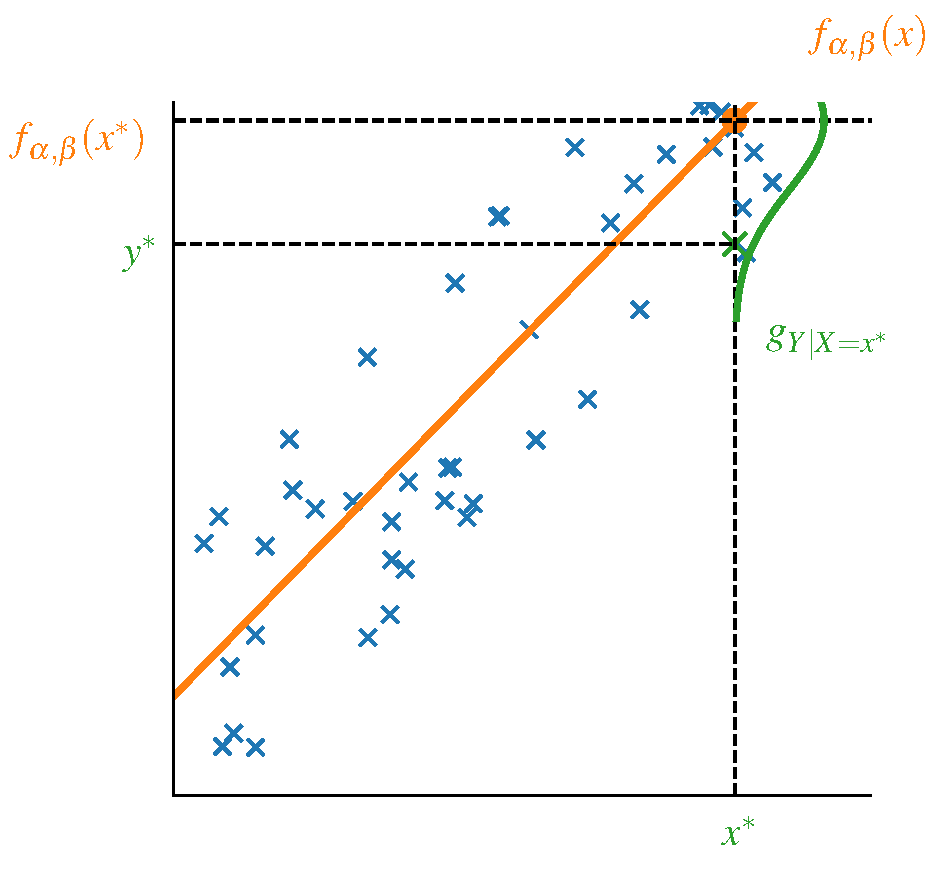
\includegraphics[width=0.6\textwidth]{figures/erm/linreg}
  \caption{Pour une observation $x^*$ donnée (ici en une dimension), la
    distribution des valeurs possibles de son étiquette est une gaussienne
    centrée en $f(x^*)$. La vraie valeur de l'étiquette est $y^*$.}
  \label{fig:linreg}
\end{figure}


\subsection{Estimation par maximum de vraisemblance $\bullet$}
\label{sec:least_squares}
Sous l'hypothèse~\eqref{eq:param_bayes}, nous pouvons estimer $\bbeta$ en
maximisant la log-vraisemblance de l'échantillon
$\left((\xx^1, y^1), (\xx^2, y^2), \dots, (\xx^n, y^n) \right), $ qui est la
réalisation d'un échantillon aléatoire constitué de $n$ copies i.i.d. de
$(X, Y)$.  En notant $g_{X,Y}$ la densité jointe de $(X, Y)$; $g_{Y|X=x}$ la
densité de $Y|X=x$; et $g_X$ la densité de $X$, cette log-vraisemblance s'écrit
\begin{equation*}
  \ell\left((\xx^1, y^1), (\xx^2, y^2), \dots, (\xx^n, y^n); \bbeta  \right)
  = \ln \prod_{i=1}^n g_{X, Y}(\xx^i, y^i) 
  = \ln \prod_{i=1}^n g_{Y|X=\xx^i}(y^i) + \ln \prod_{i=1}^n
  g_X(\xx^i)
\end{equation*}
et donc    
\begin{equation*}
  \ell\left((\xx^1, y^1), (\xx^2, y^2), \dots, (\xx^n, y^n); \bbeta  \right)
  = - \frac1{2\sigma^2} \sum_{i=1}^n \left(y^i -
    f_{\bbeta}(\xx^i) \right)^2 + \Ccal,
\end{equation*}
avec $\Ccal$ une constante par rapport à $\bbeta$, qui provient d'une part du
coefficient $\frac1{\sqrt{2\pi}}$ de la distribution normale et d'autre part
des $g_X(\xx^i)$.

Ainsi, maximiser la vraisemblance dans ce contexte de bruit gaussien centré
revient à minimiser 
\[\sum_{i=1}^n \left(y^i - f_{\bbeta}(\xx^i) \right)^2.\]
On retrouve ici la méthode des moindres carrés de l'équation~\eqref{eq:erm_parametric}.

\section{Régression linéaire}
\label{sec:linreg}
Nous allons maintenant appliquer la minimisation des moindres carrés au cas où
$\FF$ est l'ensemble des fonctions linéaires de $p$ variables.

\subsection{Formulation}
Nous choisissons une fonction de décision $f$ de la forme
\begin{equation}
  \label{eq:linear_decision}
  f: \xx \mapsto \beta_0 + \sum_{j=1}^p \beta_j x_j.
\end{equation}
Ici, $\bbeta \in \RR^{p+1}$ et donc $m=p+1$.

\subsection{Solution}
On appelle \textbf{régression linéaire} le modèle de la forme
$f: \xx \mapsto \beta_0 + \sum_{j=1}^p \beta_j x_j$ dont les coefficients sont
obtenus par minimisation de la somme des moindres carrés, à savoir :
\begin{equation}
  \label{eq:linreg}
  \argmin_{\bbeta \in \RR^{p+1}}  \sum_{i=1}^n \left(y^i - \left(\beta_0 + 
      \sum_{j=1}^p \beta_j x^i_j \right)\right)^2.
\end{equation}
  
Nous pouvons réécrire le problème~\ref{eq:linreg} sous forme matricielle, en
ajoutant à gauche à la matrice d'observations $X \in \RR^p$ une colonne de 1 :
\begin{equation}
  \label{eq:added_ones}
  X \leftarrow   \begin{pmatrix}
    1 & x_1^1 & \cdots & x_p^1 \\
    \vdots & \vdots & \cdots & \vdots \\
    1 & x_1^n& \cdots & x_p^n \\
  \end{pmatrix}.
\end{equation}

La somme des moindres carrés s'écrit alors
\begin{equation}
  \label{eq:rss_linreg}
  \text{RSS} = \left(\yy - X \bbeta\right)^\top \left(\yy -  X \bbeta\right).
\end{equation}

Il s'agit d'une forme quadratique convexe en $\bbeta$, que l'on peut donc
minimiser en annulant son gradient
$\nabla_{\bbeta} \text{RSS} = -2 X^\top \left(\yy - X \bbeta \right)$. La somme
des moindres carrés est minimale si $\bbeta$ vérifie 
\begin{equation}
  \label{eq:linreg_sol}
  X^\top X \bbeta = X^\top \yy.
\end{equation}
  
\paragraph{Solution explicite}
Si le rang de la matrice $X$ est égal à son nombre de colonnes, alors
$X^\top X$ est inversible et la somme des moindres carrés de
l'équation~\eqref{eq:rss_linreg} est minimisée pour
\begin{equation*}
  \bbeta^* = \left(X^\top X \right)^{-1} X^\top \yy.
\end{equation*}

Si $X^\top X$ n'est pas inversible, on pourra néanmoins trouver une solution
(non unique) pour $\bbeta$ en utilisant à la place de
$\left(X^\top X \right)^{-1}$ un pseudo-inverse (par exemple, celui de
Moore-Penrose) de $X^\top X$, c'est-à-dire une matrice $M$ telle que
$X^\top X M X^\top X = X^\top X.$

\paragraph{Méthode de descente}
On peut aussi (et ce sera préférable quand $p$ est grand et que l'inversion de
la matrice $X^\top X \in \RR^{p \times p}$ est donc coûteuse) obtenir une
estimation de $\bbeta$ par un algorithme à directions de descente.

\paragraph{Interprétation} La régression linéaire produit un modèle interprétable, au sens où les
$\beta_j$ permettent de comprendre l'importance relative des variables sur la
prédiction. En effet, plus $\lvert \beta_j \rvert$ est grande, plus la $j$-ème
variable a un effet important sur la prédiction, et le signe de $\beta_j$ nous
indique la direction de cet effet.

Attention ! Cette interprétation n'est valide que si les variables ne sont pas
corrélées, et que $x_j$ peut être modifiée sans perturber les autres
variables. De plus, si les variables sont corrélées, $X$ n'est pas de rang
colonne plein et $X^\top X$ n'est donc pas inversible. Ainsi la régression
linéaire admet plusieurs solutions. Intuitivement, on peut passer de l'une à
l'autre de ces solutions car une perturbation d'un des poids $\beta_j$ peut
être compensée en modifiant les poids des variables corrélées à $x_j$.

\paragraph{Remarque} % Nous avons traité ici de problèmes de \textit{régression}
% uniquement.
Nous traiterons de classification paramétrique dans la PC~5.


%-*- coding: utf-8 -*-
\section{QCM}
\paragraph{Question 1.} Quand le nombre d'observations tend vers l'infini, 
\begin{itemize}
\item[$\square$] le risque empirique d'un modèle converge vers le risque de ce modèle ; 
\item[$\square$] le risque empirique minimal converge vers le risque minimal ; 
\item[$\square$] le minimiseur du risque empirique converge vers le minimiseur du risque.
\end{itemize}

\paragraph{Question 2.} Supposons un problème de classification en 2
dimensions, avec $n$ observations. Nous considérons comme espace des hypothèses
l'ensemble des unions de $K$ cercles ($K > 0$ est fixé) : les points intérieurs
à ces cercles sont étiquetés positifs, les autres négatifs. Alors
\begin{itemize}
\item[$\square$] Il ne s'agit pas d'un modèle paramétrique.
\item[$\square$] Il s'agit d'un modèle paramétrique à $K$ paramètres.
\item[$\square$] Il s'agit d'un modèle paramétrique à $2K$ paramètres.
\item[$\square$] Il s'agit d'un modèle paramétrique à $3K$ paramètres.
\end{itemize}

\paragraph{Question 3.} Quel algorithme préférer pour entraîner une régression
linéaire sur un jeu de données contenant $n$ observations et $p$ variables :
\begin{itemize}
\item Si $n=10^5$ et $p=5$ ?
  \begin{itemize}
  \item[$\square$] Une inversion de matrice.
  \item[$\square$] Un algorithme du gradient.
  \end{itemize}
\item Si $n=10^5$ et $p=10^5$ ?
  \begin{itemize}
  \item[$\square$] Une inversion de matrice.
  \item[$\square$] Un algorithme du gradient.
  \end{itemize}
\end{itemize}

\section*{Solution}
{%
\noindent
\rotatebox[origin=c]{180}{%
\noindent
\begin{minipage}[t]{\linewidth}
\paragraph{Question 1.} Seule la première proposition est vraie. \newline

\paragraph{Question 2.} Il s'agit d'un modèle paramétrique et nous avons besoin
de $3K$ paramètres pour déterminer les coordonnées de $K$ cercles (coordonnées
du centre + rayon). \newline

\paragraph{Question 3.}  Lorsque la matrice $X^\top X$ (de dimensions
$p \times p$) est de petite taille (peu de variables), on pourra utiliser un
algorithme d'inversion de matrice. Sinon, un algorithme du gradient sera plus
approprié.
\end{minipage}%
}%

%%% Local Variables:
%%% mode: latex
%%% TeX-master: "../../sdd_2025_poly"
%%% End:



%%% Local Variables:
%%% mode: latex
%%% TeX-master: "../sdd_2025_poly"
%%% End: